\documentclass[a4paper]{article}

\usepackage{natbib}
\usepackage[english]{babel}
\usepackage[utf8]{inputenc}
\usepackage{amsmath}
\usepackage{graphicx}
\usepackage[colorinlistoftodos]{todonotes}

\usepackage{tikz}
\usetikzlibrary{math,fpu,calc,fit,mindmap,backgrounds,positioning}

\usepackage{xspace}
\newcommand{\eg}{e.g.\xspace}
\newcommand{\etal}{et al.\xspace}
\newcommand{\ie}{i.e.\xspace}
\newcommand{\etc}{etc.\xspace}
\newcommand{\vs}{\textit{vs.}\xspace}

\graphicspath{{figs/}}

\title{The robot who pretend-played with me}


\author{Séverin Lemaignan, Tony Belpaeme}

\date{\today}

\begin{document}
\maketitle

Alternative titles:

\begin{itemize}
    \item Can I have real fun playing with my robot?
    \item A Window Onto Your Mind: Playful Robots Leveraging Attention to
        Predict Actions
    \item Playing Like your Friend: Dealing with the High Dimensionality of
        Real-World Social Dynamic

\end{itemize}

\begin{abstract}

    This article presents how attention tracking enables a robot to first automatically segment
    a social interaction into meaningful situations (\emph{situation awareness}), and
    second, to predict the participants' actions.

    We study this effect in a high-dimensional social interaction situation based on
    free dramatic play: pairs of children (4-7 years old) or robot and child are
    invited to freely interact with characters and items on an interactive
    table, telling and acting stories with no explicit preset goal.
    
    Although the actions performed by the children are not known beforehand, our
    approach allows the robot to segment on the fly the interaction flow into
    episodes whose main focus can be predicted and used to generate pro-social
    behaviours.

\end{abstract}


\section{Introduction}

\subsection{Mutual Modelling: Theoretical Background}

Human social dynamics rely upon the ability to effectively attribute beliefs,
goals and percepts to other people. This set of meta-representational abilities
shapes what is called a theory of mind (ToM) or the ability to mentalize, and
leads to mutual modelling: the reciprocal ability to establish a mental model of
the other. This lays at the core of human interactions: normal human social
interactions depend upon the recognition of other sensory perspectives, the
understanding of other mental states, and the recognition of complex non-verbal
cues of attention and emotional state. As such, adapting and transferring these
cognitive skills to social robots is an important research objective.


Understanding and predicting one's behaviour.

An integrated theory of social cognition, applicable to robots

A principled yet practical approach to social cognition for artificial intelligence

\subsubsection{Pretense}

A second direction for the 'meta-cognitive foundations of mind modelling' is
Leslie's paper on the role of pretense~\cite{leslie1987pretense}.

\subsubsection{Surface Alignment vs Deep Grounding}

Pickering and Garrod~\cite{pickering2006alignment} argue that mutual understanding
starts mostly with a \emph{superficial alignment} at the level of the linguistic
representations, due to priming mechanisms, and that this local alignment may --
in some cases -- lead to a \emph{global alignment} of the semantic level
(\emph{deep grounding}).  For these authors, the convergence in dialogue, and
even the repair of some misunderstandings, is explained by this mimetic behavior
more than by a monitoring of each other's knowledge:

\begin{quote}
[\ldots] interlocutors do
not need to monitor and develop full common ground as a regular, constant
part of routine conversation, as it would be unnecessary and far too costly.
Establishment of full common ground is, we argue, a specialized and
non-automatic process that is used primarily in times of difficulty (when
radical misalignment becomes apparent).~\citep[p.179]{pickering2006alignment}
\end{quote}


analysis of behavioural alignment between partners (via
metrics like the recently proposed \emph{Individual Motor
Signature}~\cite{slowinski2016dynamic})

\subsubsection{Theory of Mind}

We previously covered the state of the research on theory of mind in social
robotics~\cite{lemaignan2015mutual}.

In~\cite{scassellati2002theory}, Scassellati gave
an initial account of Leslie's and Baron-Cohen's respective models of the
emergence of a theory of mind (we discuss them below) from the perspective of
robotics, but reported implementation work was limited to simple perceptual
precursors (like face detection or color saliencies detection). Since then,
research in this field has been focused on applications relying on Flavell's
\emph{Level 1}~\cite{flavell1977development} perspective-taking, \ie
perspective-taking that only requires perceptual abilities (``\emph{I see (you do
not see the book)}''), and actually mostly limited to visual perception (relevant
work include Breazeal~\cite{breazeal2006using}, Trafton~\cite{Trafton2005} and
Ros~\cite{Ros2010}).

Based on perspective taking \emph{Level 1} alone, Breazeal
\etal\cite{breazeal2009embodied} and Warnier \etal\cite{warnier2012when}
successfully tackled the classical hallmark of theory of mind, the false belief
experiment (also known as the ``Sally and Anne'' experiment, introduced
by~\cite{wimmer1983beliefs}, original experimental setting
by~\cite{baron1985does}). They demonstrated complete human-robot interaction
scenarios where robots recognize and handle false belief situations in dyadic or
triadic interactions, and exhibit helping behaviours that account for the
missing/false beliefs of the human partners.

\cite{devin2016implemented}

\subsubsection{Connections vs. representations}
\label{connection-representation}

In~\cite{flavell1990developmental}, Flavell relates perspective taking
\emph{Level 1} to establishing \emph{cognitive connections} (I see, I hear, I
want, I like, I fear...), in contrast to perspective taking \emph{Level 2} that
relates to manipulating \emph{representations}.  This is exemplified by
\emph{appearance-reality} tasks, like the \emph{elephant mask} experiment
proposed in~\cite{flavell1990developmental}: 3-years old children are not able
to tell that an experimenter hidden behind a large elephant mask but who speaks
normally \emph{looks} like an elephant, \emph{sounds} like the experimenter, and
\emph{really is} the experimenter.  It appears that, while those children are
able to explicitly manipulate cognitive connections (they know for instance that
these are largely independent of each other and that they can evolve over time)
and know as well that their own connections are independent of those of other
people, they do not think that one concept can \emph{seriously} (\ie non
playfully) hold several, possibly conflicting, representations.

\subsection{Attention in Robotics}


\section{Methodology: Social Interaction during Free Play}


The study of the emergence of social behaviour is often intrinsically limited by
the nature of the experimental tasks. We introduce a new
experimental paradigm based on free play interactions. Where traditional
socio-cognitive tasks are either toy scenarios (\ie they do not adequately
mirror real-world situations) or simple, constrained tasks that do not reflect
the complexity and dynamics of real-world interactions, free play social
interactions exhibit a rich set of natural cognitive and social dynamics that
are desirable for this research.

\begin{figure}
    \centering
    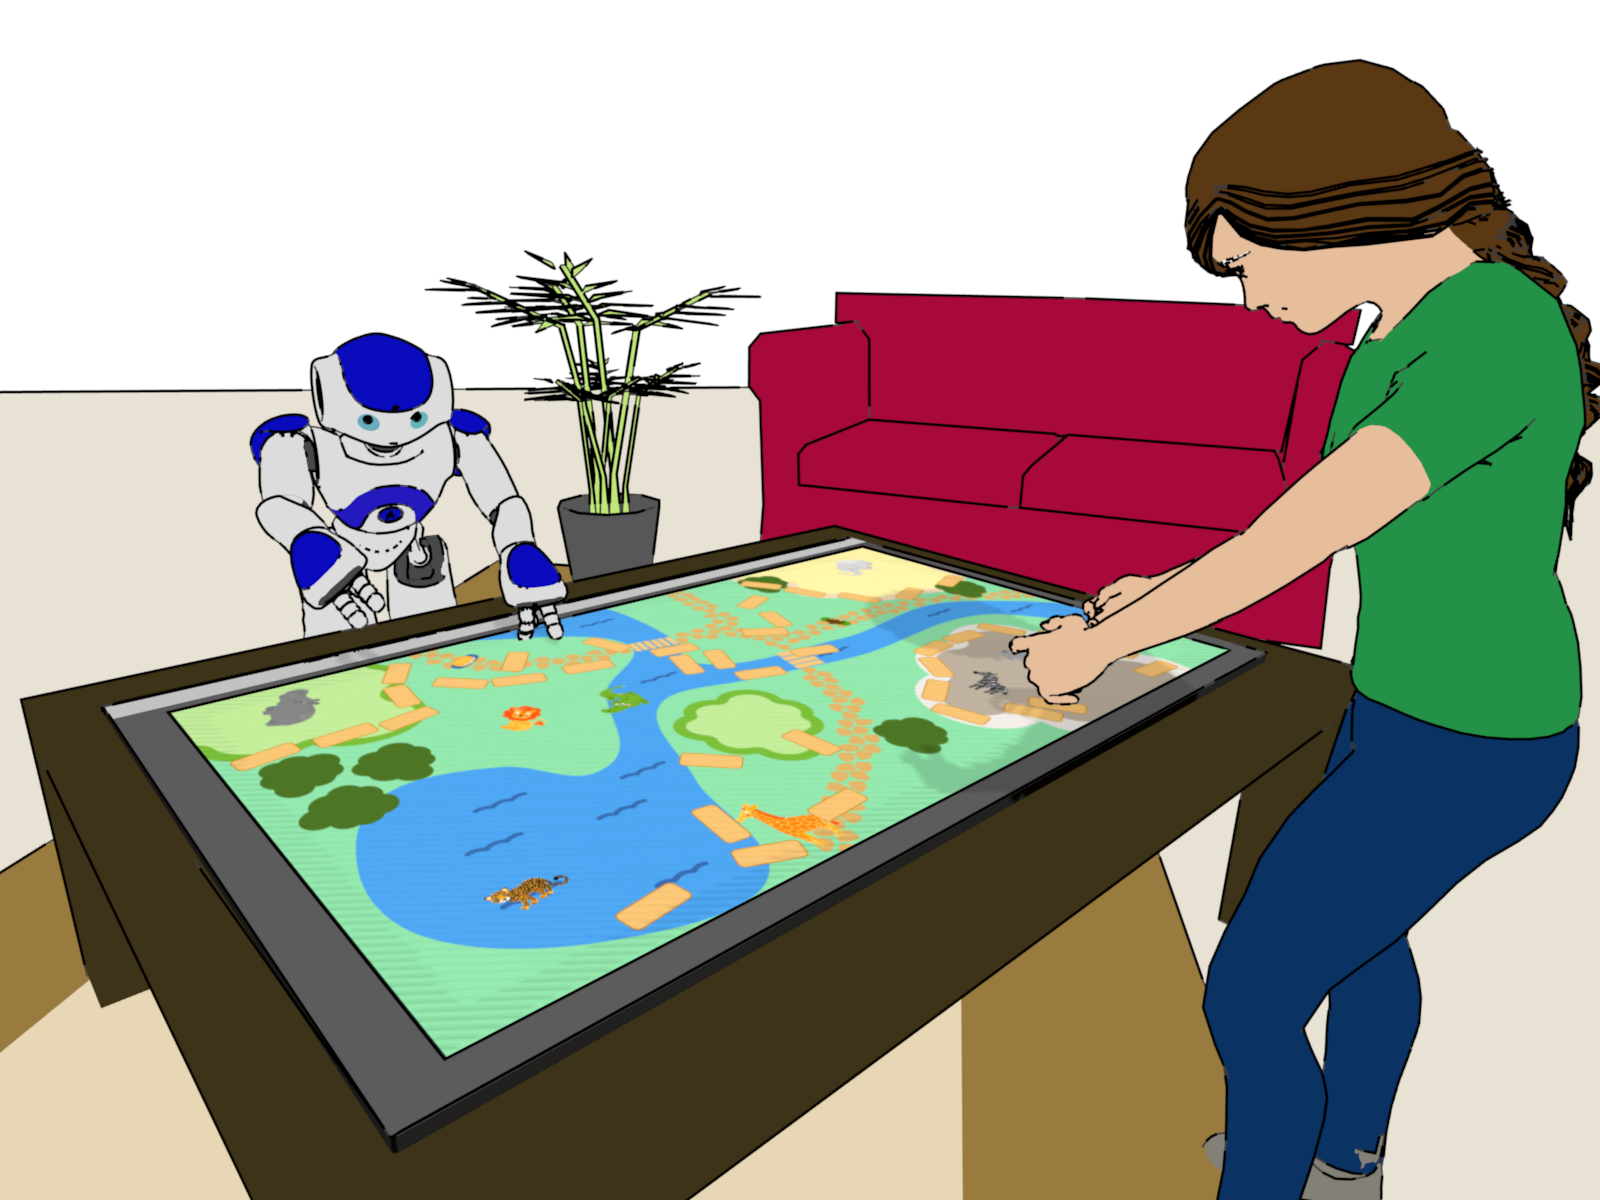
\includegraphics[width=0.9\linewidth]{setup.png}
    \caption{The free play social interactions sandbox}
    \label{fig|setup}
\end{figure}

To mitigate the technical challenges presented by free play interactions (like
high dimensionality and uncertainties), we have developped a  \emph{free
play sandbox}~\ref{fig|setup}: open-ended and non-directive activities, yet sufficiently
defined to be reproducible; focus on abstract socio-cognitive facets (robot
perception and manipulation are simplified); well suited for qualitative and
quantitative analysis using metrics like Słowinski’s Individual Motor Signature
(for behavioural alignment), Ballard’s coding of children’s free-play
interactions, with-me-ness (for assessment of co-engagment).


\subsection{Free play task}

\begin{figure}
    \centering
    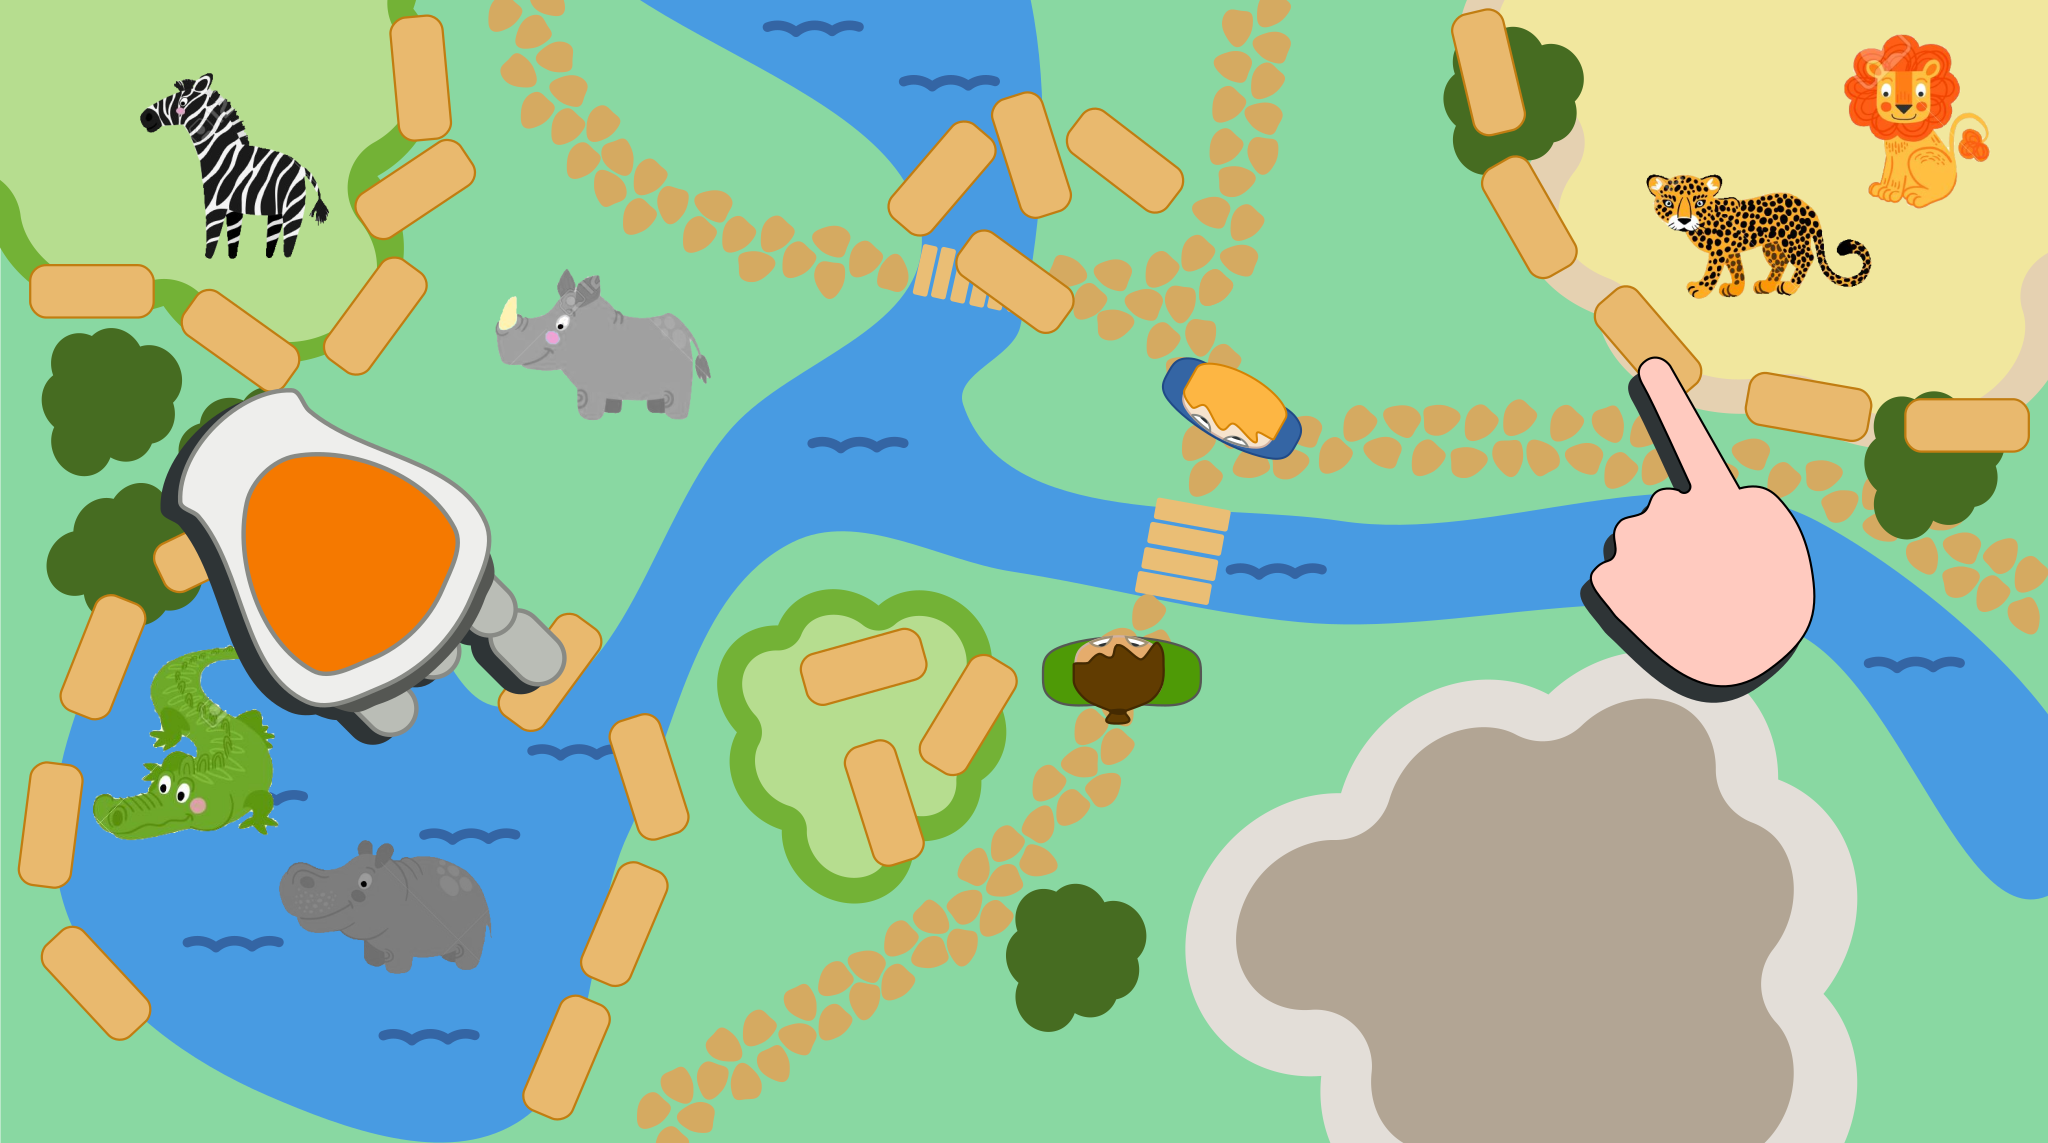
\includegraphics[width=0.9\linewidth]{sandbox}
    \caption{Example of a game situation: the child and the robot `build'
    together a zoo. The animals and the blocks can be dragged over the whole
    play area, while the background picture is static and purely decorative.}
    \label{fig|sandbox}
\end{figure}


\begin{figure}
    \centering
    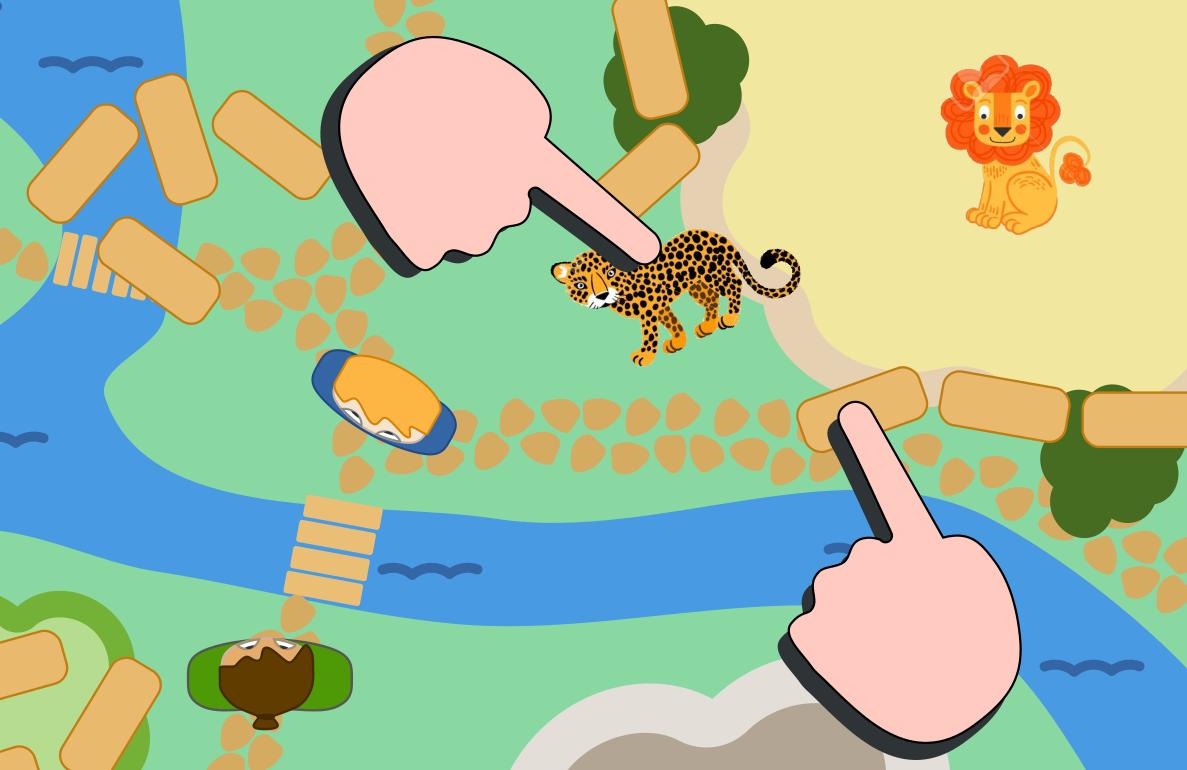
\includegraphics[width=0.7\linewidth]{sandbox-release-cheetah}
    \caption{Possible play situation: the child decides to release the cheetah
    and creates a story where the cheetah scares away the visitors.}
    \label{}
\end{figure}

\subsection{Data Analysis}

\begin{figure}
    \centering
    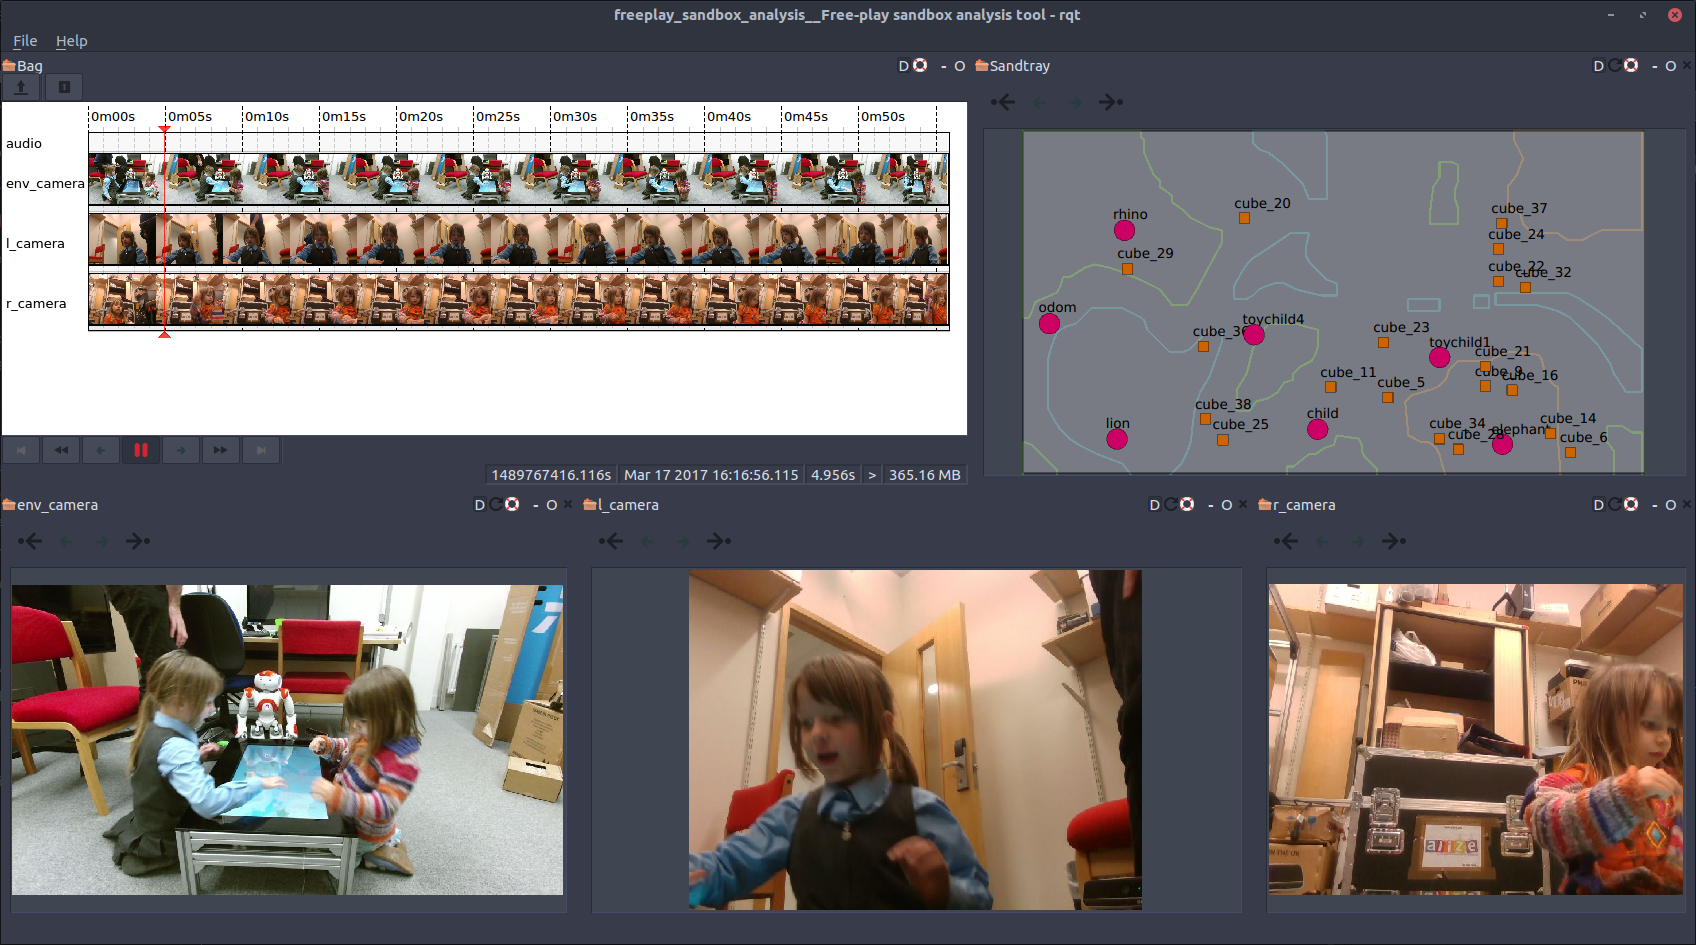
\includegraphics[width=\linewidth]{analysis}
    \caption{Screenshot of the interaction analysis tool: faces of the two
    children are recorded, as well as any interaction occuring on the
    interactive table.}
    \label{fig|analysis}
\end{figure}

\section{Discussion: Towards a Model of Socio-Cognitive Awareness for Robots}

\subsection{The classical approach}


Symbolic approaches to social cognition work by first building a mental model of the
interacting humans. This is typically done by a combination of 3D situation
assessment (the robot builds and update a semantic 3D model of its environment)
and visual perspective taking (based on the estimation of the pose of the human
head). This permits the computation of allocentric, and more importantly,
egocentric spatial relations between the spatial entities in the environment
(we call it \emph{social situation assessment}).

This geometric computations are then turned into symbolic representations,
typically using logical statements (embedded in logic
programming~\cite{tenorth2009knowrob} or ontologies~\cite{lemaignan2010oro}).

The robot creates and continuously updates one symbolic model per
agent~\cite{lemaignan2010oro}. These models are then used by other cognitive
processes (task planning, dialogue, task execution supervision) that are
designed to take advantage of the agents' knowledge models to produce
socially-aware behaviours: for example, the task planner may plan manipulation
task using only entities visible to the human~\cite{lallement2014hatp}, or the
dialogue manager may use the specific knowledge model of the speaker to
interpret the speech, avoiding grounding ambiguities that might otherwise
occur~\cite{lemaignan2011grounding}.

This works well as long as we limit ourselves to the manipulation of the results
of visual perspective taking. However, one intuitively recognizes that social
modelling goes indeed beyond computing what the human perceives or does not
perceive. This has been clearly recognized in developmental psychology, for
instance with Flavell's distinction between \emph{cognitive connections} on one
hand, and \emph{mental representations} on the other hand (we will come back to
Flavell's \emph{connection-representation} account in
section~\ref{connection-representation}). Now, if we are to model someone else's
mind beyond a naive geometric model of their perception, we indeed enter the
realm of \emph{representations}. What are they? How to access them? How to
represent and manipulate them? These three questions lay at the core of this
work, and as such we effectively take over the point we previously made
in~\cite{lemaignan2015mutual}:  we ultimately want to come up with a
meta-representational cognitive system to \emph{represents
representations} (including representations of \emph{false} beliefs or unknown
facts, \ie suppositions).

We must immediately clarify that, even though this goal may seem to pre-suppose
\emph{symbolic} meta-representations, this is not the case: at that stage, we do
not have evidence that a particular kind of computational structure may better
support the representation and manipulation of mental representations.

[What is not adequately solved by current techniques?]

[give concrete examples of social situations that are not easily achieveable
with current (symbolic or not) approaches]

[this examples should be turned into predictions for what our proposal should be
able to achieve]



\subsection{Phenomenal \vs Access Consciousness}

Neuroscientist view: Block's proposal of two kind of consciousness~\cite{block1996can}:
\emph{phenomenal} consciousness as the raw inner experience; \emph{access}
consciousness as the more abstract, cognitive ability to think about and report
on those experiences.

Does this map to the traditional sub-symbolic/symbolic divide that we observe in
artificial intelligence, and in particular in robotics?

The \emph{phenomenal consciousness} would then be the immediate raw perceptual
inputs: video streams from cameras, readings for torque and force sensors, joint
positions, etc.

The \emph{access consciousness} would typically be the symbolic representation
of these inputs.


We must however keep in mind that there is likely no such rigid dichotomy
between phenomenal consciousness and access consciousness. It is rather a
continuum of processing~\citep[p.55]{graziano2013consciousness}

Recursivity of consciousness: if I'm looking at a green apple, my cognitive
machinery can decide and report that I'm aware of green. I can also be aware of
the deciding and aware of the reporting~\citep[p.55]{graziano2013consciousness}.

\subsection{From Social Attention to Social Modelling: the Attention Schema Theory}

The hypothesis that we hereafter develop and turn into a cognitive model is the
following: \textbf{mental representations are snapshots of awareness, awareness being
itself a label for the memory-mediated process of attention}.

This extends to social cognition: \textbf{modelling others' mental representations is
taking snapshots of their current state of awareness}. As we do not have direct
access to others' process of attention, it has to be mediated. We suggest that
\textbf{modelling other's state of awareness is mediated by one's own
attentional system, through joint attention mechanisms}.


Our approach draws form the \emph{Attention Schema Theory}, proposed by
Grazino~\cite{graziano2013consciousness}.

What awareness can do? ``the brain \emph{does} attention, but \emph{knows}
awareness'': as such, ``awareness can in principle be verbally reported''.



Associative Memory as an Informational Proxy for the Attention System


\begin{enumerate}
    \item Perceptual inputs feed in an associative memory

    \item the resulting set of pre-activated units is the current
        \emph{focus of attention} -- this step may require dimensionality
        reduction techniques

    \item According to the Attention Schema Theory, by \emph{explicitely}
        labelling the activated and pre-activated units as being attended, we
        make the robot \emph{aware} of the corresponding phenomenons.

    \item The labelling occurs by the mean of a symbolic association within a
        semantic network (ontology)

\end{enumerate}

\paragraph{Attention}

Modelled as a \emph{Biased Competition Model of
Attention}~\cite{desimone1995neural}.
Implemented using a particular \emph{Associative Memory Network} with an
additional top-down biasing mechanism.

\paragraph{Memory-mediated Attention}

\emph{Attention} is modelled as the set of activated units in an associative
memory network.


Interplay between multi-modal social cues on one hand, and priming of previously activated physical
entities (objects, agents) and 

Attention


\begin{figure}[h!]
    \centering
        \resizebox{0.7\linewidth}{!}{%
        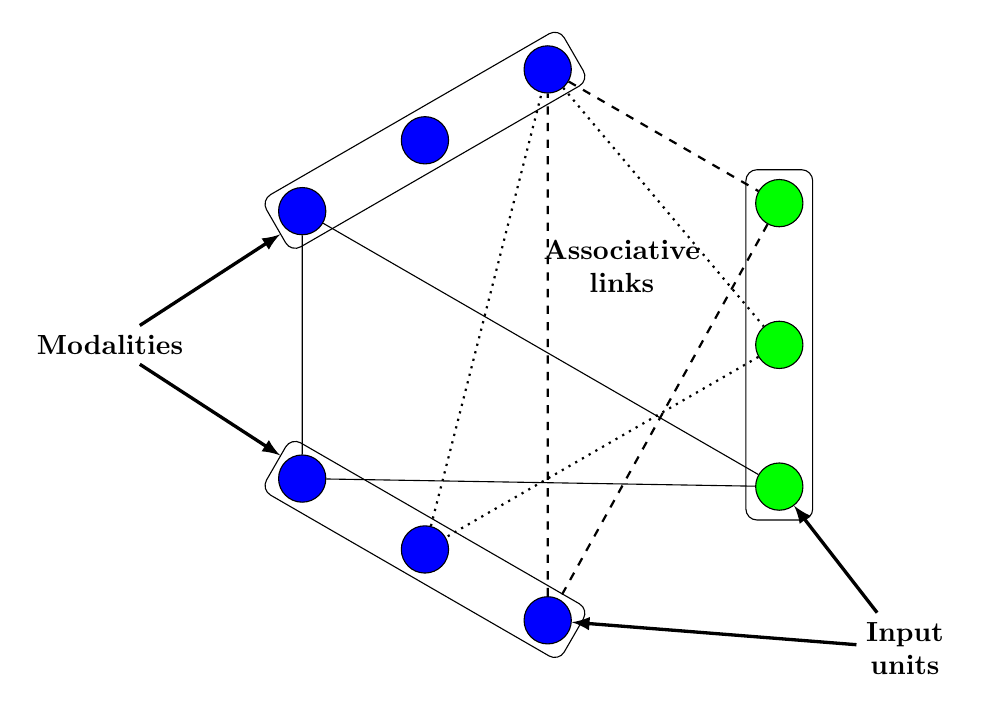
\begin{tikzpicture}[
                >=latex,
                every edge/.style={draw, very thick},
                every node/.style={font=\bf,align=center},
                input/.style={draw,circle, inner sep=0pt,minimum size=0.6cm}
            ]

            % draw the units
            \foreach \x [count=\xi] in {0, 120, 240}
                \foreach \y [count=\yi] in {-.6, 0, .6}
                    %\node[input, ball color=orange!\x!blue] at ($(\x:3)!\y!90:(0,0)$) (i\xi\yi) {};
                    \node[input, fill=blue!\x!green] at ($(\x:3)!\y!90:(0,0)$) (i\xi\yi) {};

            \node[draw,rounded corners, fit=(i11)(i12)(i13)] (modA) {};
            \node[draw,rounded corners, rotate fit=120,fit=(i21)(i22)(i23)] (modB) {};
            \node[draw,rounded corners, rotate fit=60,fit=(i31)(i32)(i33)] (modC) {};

            \node at (180:5.5) {Modalities} edge[->] (modB) edge[->] (modC);
            \node at (-40:6) {Input\\units} edge[->] (i13) edge[->] (i31);

            \path[draw,dashed, thick]  (i23) -- (i11) -- (i31) -- (i23);
            \path[draw,dotted, thick] (i23) -- (i12) -- (i32) -- (i23);
            \path[draw] (i21) -- (i13) -- (i33) -- (i21);

            \node at (1,1) {Associative\\links};
        \end{tikzpicture}
    }

    \caption{Associative Memory Network}
    \label{blabla}
\end{figure}



\paragraph{Biasing Mechanisms}

Biasing competition~\cite{beck2009top}

The bottom-up biasing mechanism follows naturally from the structure of the
associatve memory model: a strong and long activation of a perceptual input
leads to the activation of the corresponding unit in the memory network and the
suppression of competing inputs.

The top-down mechanism is to be invented :-)
It should enable high-level decisional processes to effectively suppress (or
reinforce) units. The \emph{nature} and \emph{representation} of these
high-level processes is unclear, but might be of symbolic nature.



\paragraph{Social Attention}

What do we call the \emph{attention state} of a partner?


Grazino~\cite{graziano2013consciousness}: ``the mental machinery to model
someone else attentional state is the same as the one used for oneself.''

``In both case, the purpose is understanding and predicting one's behaviour.''

Cues from which we reconstruct someone else's attentional state (from Graziano):
\begin{itemize}
    \item gaze direction
    \item facial expression
    \item body language
    \item prior knowledge of person
    \item location of salient objects
\end{itemize}

\subsection{What Does the Model Predict?}

\paragraph{Protodeclarative pointing}

Protoimperative vs protodeclarative pointing~\cite{baron1986perceptual}

\paragraph{Behavioural Alignment}
\paragraph{Verbalization of the (Social) Attentional Process}
\paragraph{False-beliefs}


Picture ordering protocol, with \emph{mechanical}, \emph{behavioural} and
\emph{intentional} sequences~\cite{baron1986mechanical}

\paragraph{Symbol Grounding}

\paragraph{Recursive Awareness}

I can describe what I'm aware of, I can also recursively be aware I'm describing
my state of awareness, and I can verbalize this second order awareness.

This should work \emph{Attention Schema} theory because the attention schema
is seen as a regular sensory
representation~\citep[p.55]{graziano2013consciousness}.

\paragraph{Adapted behaviour to the interacting agent}

A robot facing a baby, a 3 years old, a 5 years old, a 13 years old or an adult
should behave differently.


\paragraph{Parten's stages of play}


\section{Conclusion}

\bibliographystyle{plain}
\bibliography{biblio}

\end{document}
